%!TEX TS-program = xelatex
\documentclass{report}

%%%%%%%%%%%%%%%%%%%%%%%% Шрифты %%%%%%%%%%%%%%%%%%%%%%%%%%%%%%%%%
\usepackage{fontspec}         % пакет для подгрузки шрифтов
\setmainfont{Arial}   % задаёт основной шрифт документа

% Команда, которая нужна для корректного отображения длинных тире и некоторых других символов.
\defaultfontfeatures{Mapping=tex-text}

% why do we need \newfontfamily:
% http://tex.stackexchange.com/questions/91507/
\newfontfamily{\cyrillicfonttt}{Arial}
\newfontfamily{\cyrillicfont}{Arial}
\newfontfamily{\cyrillicfontsf}{Arial}

\usepackage{polyglossia}      % Пакет, который позволяет подгружать русские буквы
\setdefaultlanguage{russian}  % Основной язык документа
\setotherlanguage{english}    % Второстепенный язык документа

%%%%%%%%%% Работа с картинками %%%%%%%%%
\usepackage{graphicx}                  % Для вставки рисунков
\usepackage{graphics}

%%%%%%%%%% Гиперссылки %%%%%%%%%%

\usepackage{hyperref}
\hypersetup{
    unicode=true,           % позволяет использовать юникодные символы
    colorlinks=true,       	% true - цветные ссылки, false - ссылки в рамках
    urlcolor=blue,          % цвет ссылки на url
    linkcolor=black,        % внутренние ссылки
	pdfnewwindow=true,      % при щелчке в pdf на ссылку откроется новый pdf
	breaklinks              % если ссылка не умещается в одну строку, разбивать ли ее на две части?
}

%%%% Оформление %%%%%%%
\usepackage[14pt]{extsizes} % Возможность сделать 14-й шрифт

% размер листа бумаги
\usepackage[paper=a4paper,top=10mm, bottom=10mm,left=35mm,right=35mm,includefoot,includehead]{geometry}

\usepackage{setspace}
\setstretch{1}  % Межстрочный интервал
\setlength{\parindent}{0cm} % Красная строка.

\setlength{\parskip}{4mm}   % Расстояние между абзацами
% Разные длины в латехе https://en.wikibooks.org/wiki/LaTeX/Lengths

\flushbottom                            % Эта команда заставляет LaTeX чуть растягивать строки, чтобы получить идеально прямоугольную страницу
\righthyphenmin=2                       % Разрешение переноса двух и более символов
\widowpenalty=300                     % Небольшое наказание за вдовствующую строку (одна строка абзаца на этой странице, остальное --- на следующей)
\clubpenalty=3000                     % Приличное наказание за сиротствующую строку (омерзительно висящая одинокая строка в начале страницы)
\tolerance=1000     % Ещё какое-то наказание.

\usepackage{fancyhdr} % Колонтитулы

\usepackage{nameref}

\renewcommand{\headrulewidth}{0.2pt}  % Толщина линий, отчеркивающих верхний
	\cfoot{Школа Чародейства и Волшебства "Хогвартс"}
	\lhead{ПРИЛОЖЕНИЕ \Asbuk{section}}
 	\chead{\nameref{\thesection}}
 	\rhead{\thepage} % номер страницы
	
% Редактирование заголовков
\usepackage{titlesec}  

\titleformat{\section}
	 {\bfseries\Large}
	 {\thesection}{0.5 em}{}

\renewcommand{\thesection}{Приложение \Asbuk{section}:}


\begin{document} % конец преамбулы, начало документа

\pagestyle{empty}

\begin{center}

\includegraphics[width=10cm, height=6cm, keepaspectratio]{hogwarts.png}
\end{center}

\vspace{1cm}

{\fontsize{12}{1}\selectfont Мистеру Константинову}

\vspace{2.5cm}

Дорогой Мистер Константинов, 

Мы рады сообщить, что Вам предоставлено место в Школе Чародейства и Волшебства "Хогвартс". До 31 июня Вам необходимо послать к нам ушастую сову, дабы сообщить о факте получения данного письма. 

В 11 часов 31 августа Вам необходимо, вместе с предметами, указанными в Приложении А, оказаться на Курском вокзале и как можно увереннее вбежать в стену левее касс поездов дальнего следования. Мы в Вас верим.

Главное --- ничего не бойтесь.

Искренне Ваша,

{\fontsize{20}{1}\selectfont\fontspec{Hijrnotes PERSONAL USE ONLY 01}{Minerva McGonagall}}

Минерва МакГонагалл \\
заместитель директора

\vfill 
\begin{center} 
Школа Чародейства и Волшебства "Хогвартс" \\ 
{\fontsize{12}{1}\selectfont \href{http://synergy.ru/}{Ссылка на сайт Школы}} 
\end{center}

\newpage

\pagestyle{fancy}

\section{Список необходимых книг и предметов}\label{\thesection}

\begin{itemize}
\renewcommand{\labelitemi}{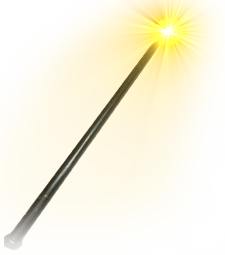
\includegraphics[scale=0.05]{Wand_logo.png}}
  \item Волшебная палочка
  \item Чугунный котёл
  \item Книга «Фантастические звери: места обитания». \\ Автор~---~Ньют Саламандер
  \item Рогатка и камушки для охоты на "Сами-знаете-кого"
\end{itemize}

\newpage

\section{Список изучаемых предметов}\label{\thesection}

\begin{itemize}
\renewcommand{\labelitemi}{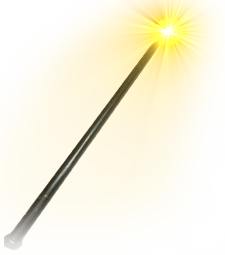
\includegraphics[scale=0.05]{Wand_logo.png}}
  \item Зельеварение
  \item Заклинания
  \item Как съесть все вкусные «Берти Боттс» и заставить всех тебя ненавидеть
\end{itemize}

\end{document}

